%%%%%%%%%%%%%%%%%%%%%%%%%%%%%%%%%%%%%%%%%%%%%%%%%%%%%%%%%%%%%%%%%%%%%%
% How to use writeLaTeX: 
%
% You edit the source code here on the left, and the preview on the
% right shows you the result within a few seconds.
%
% Bookmark this page and share the URL with your co-authors. They can
% edit at the same time!
%
% You can upload figures, bibliographies, custom classes and
% styles using the files menu.
%
%%%%%%%%%%%%%%%%%%%%%%%%%%%%%%%%%%%%%%%%%%%%%%%%%%%%%%%%%%%%%%%%%%%%%%

\documentclass[12pt]{article}

\usepackage{sbc-template}

\usepackage{graphicx,url}

%\usepackage[brazil]{babel}   
\usepackage[utf8]{inputenc}  

     
\sloppy

\title{Paralelização para memória distribuída com MPI}

\author{Bruno C. P. D. Rosa, Cristofer A. Oswald}

\address{Departamento de informática 
  \\Centro de Tecnologia -- Universidade Estadual de Maringá
  (UEM)\\
  Maringá -- PR -- Brasil
}

\begin{document} 

\maketitle
     
\begin{resumo} 
  A busca continua por mais poder computacional e eficiência levou a inevitável ascensão das arquiteturas paralelas, que atualmente dominam o mercado e estão presentes em todo tipo de dispositivo. Estas mudanças também afetaram profundamente o modelo de programação, causando uma troca de paradigma. Programar paralelamente se tornou crucial para o desenvolvimento de aplicações capazes de utilizar o hardware moderno. Neste trabalho investigamos o desempenho de diversos métodos de programação paralela disponíveis atualmente comparando-os entre sí utilizando como objeto de experimentação programas de alto desempenho.
\end{resumo}


\section{Introdução}
Na história da ciência da computação os avanços no hardware sempre foram os maiores impulsionadores do aumento do poder computacional, o mesmo software simplesmente roda mais rápido à medida que os processadores apresentam uma maior velocidade de processamento, durante anos cientistas e desenvolvedores de software contaram com isto para atingirem seus objetivos. Esse impulso, porém, diminuiu desde 2003 devido a questões de consumo de energia e dissipação de calor, que limitaram o aumento da frequência do clock e o nível de tarefas que podiam ser realizadas em cada período de clock dentro de uma única CPU \cite{kirk2011programming}. A indústria de microprocessadores respondeu a estas limitações com a mudança do paradigma dominante nas arquiteturas de computadores, que agora são as arquiteturas paralelas, principalmente sob a forma de processadores multinúcleos.

Um dos métodos de paralelização mais antigos é a paralelização para execução em cluster, onde cada fluxo de execução é alocado em uma máquina diferente num cluster de computadores. Assim cada máquina se torna responsável por parte do processamento, esta estratégia já era utilizada muito antes do surgimento dos processadores multinúcleos. Este modelo, denominado programação paralela com memória distribuída, apresenta vantagens e desvantagens quando comparado ao modelo de paralelização com memória compartilhada. Neste trabalho exploramos os aspectos deste modelo utilizando a técnica de passagem de mensagens como solução para comunicação entre os dispositivos, analisando seus pontos fortes e fracos.


\section{Projeto} \label{sec:projeto}

O programa de alto desempenho \textit{Fast} escrito na linguagem C, foi escolhido para ser usado como objeto de experimentação deste trabalho. A versão original do programa é uma implementação paralela do algoritmo utilizando a técnica de paralelização de laços com a ferramenta \textit{OpenMP}. \textit{Fast} faz parte do CAP benchmark \cite{souza2017cap} um benchmark desenvolvimento com o objetivo principal de testar o desempenho e o gasto de energia em processadores multinúcleos. O número de fluxos de execução concorrentes e o tamanho do problema são parâmetros de execução do programa.

\textit{Fast}, acrônimo do inglês \textit{Features from Accelerated Segment Test} implementa um método para detecção de cantos em imagens seguindo o padrão estêncil paralelo. É comumente usado para extrair características e mapear objetos em tarefas de visão computacional. Em sua execução, um circulo de 16 pixels é utilizado para testar se um ponto \(p\) candidato é um canto ou não. Um valor inteiro de 1 a 16 é atribuído para cada pixel no circulo em ordem horária. Se todos os \(N\) pixel contínuos do circulo são mais claros que a intensidade do pixel candidato \(p\) somado a um valor limiar \(t\) ou todos mais escuros que a intensidade de \(p - t \), então \(p\) é classificado como um canto.
	
Para avaliar o desempenho do programa no modelo paralelo com memória distribuída foi implementada uma versão que utiliza a técnica de passagem de mensagens através de MPI. Uma implementação MPI (\textit{Message Passing Interface}) é uma API para envio de mensagens juntamente de protocolos e especificações semânticas sobre seu funcionamento \cite{Lusk96ahigh-performance}. A implementação MPI utilizada é a Open MPI, uma versão desenvolvida e mantida por um consórcio de parceiros acadêmicos, pesquisadores e outros interessados.



Todos os códigos foram compilados com otimização O3 e executados em um computador intel i5-6300HQ com 8Gb de memória DDR4 rodando o sistema operacional Ubuntu 18.04 LTS.

\section{Avaliação}

A metodologia de avaliação adotada compreende o uso de ferramentas de análise aprofundada do desempenho da execução dos programas, busca-se assim coletar dados como número de instruções executadas, ciclos de clock, trocas de contexto, acessos a cache (hit/miss) e resultados da previsão de desvios durante a execução. Para garantir resultados mais precisos e evitar possíveis falsas conclusões o experimento realizado contempla onze execuções de cada implementação com a entrada de maior tamanho disponível, sendo que a primeira tem a finalidade de aquecer a cache e o melhor e pior resultado são descartados, assim os dados utilizados na avaliação são as médias das 8 execuções restantes.

\subsection{Linked List}
A avaliação do \textit{Linked List} tem como objetivo comparar o desempenho das diferentes técnicas de paralelização selecionadas, ignorando porém a análise do speedup na execução com variação no número de fluxos de execução, isto porque a velocidade de execução deste programa não se beneficia significativamente do aumento do número de fluxos paralelos devido a sua natureza. Implementar as versões paralelas deste programa teve uma função mais didática quanto ao aprendizado das técnicas de paralelização, entretanto, pode-se ainda utilizar os resultados de suas execuções para comparar superficialmente o desempenho das diferentes implementações utilizando o número total de operações processadas durante cada execução do programa, com duração fixa de cinco segundos.

\begin{figure}[ht]
\centering
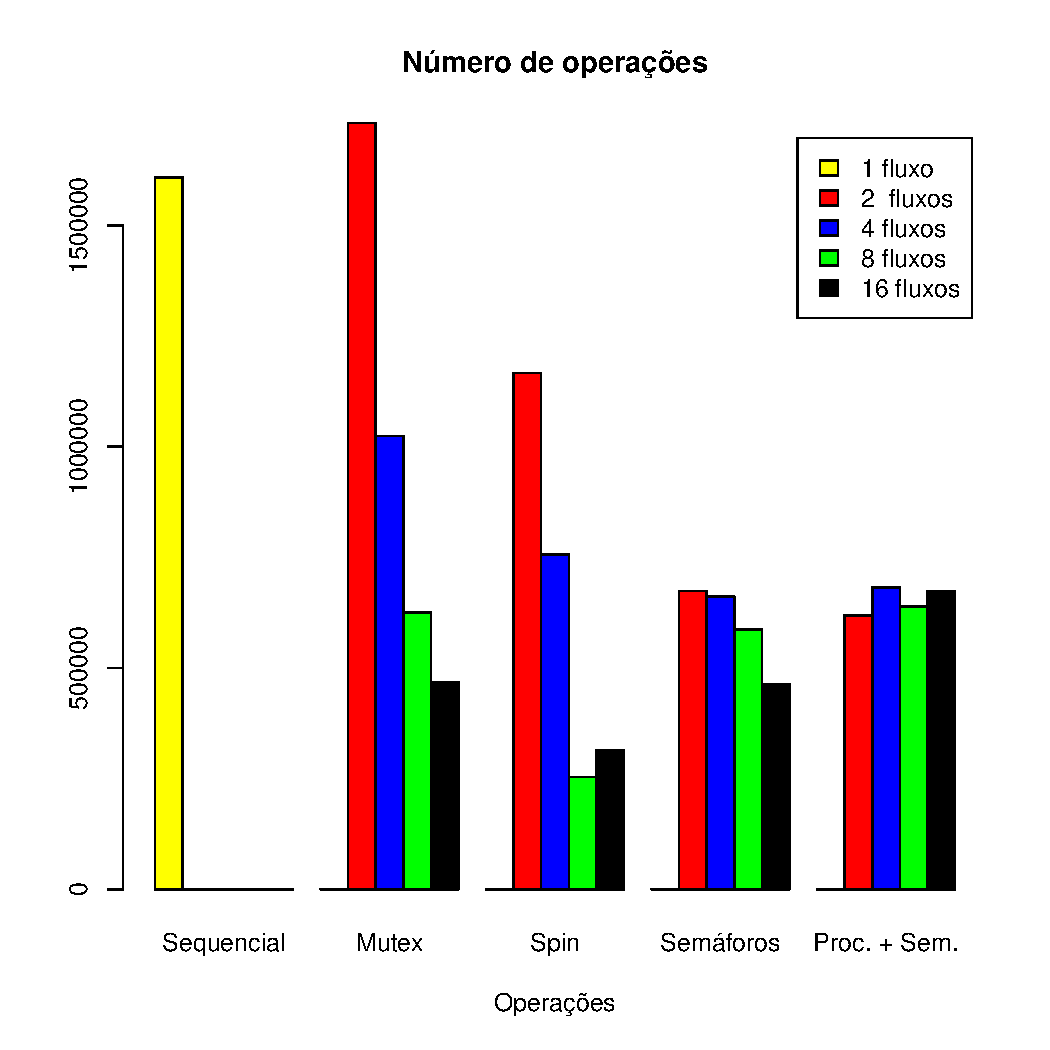
\includegraphics[width=.5\textwidth]{l_ops.pdf}
\caption{Gráfico de análise dos resultados do Linked List}
\label{fig:grafico1}
\end{figure}

Apesar de parecer contraditório os resultados obtidos são justificados através da natureza do programa Linked List que, para garantir a integridade de seus dados durante tempo de execução, não é capaz de gerenciar diversos fluxos de execução de forma a rodarem de maneira realmente paralela, isto por que cada operação realizada, entre inserir novos elementos, remover ou até mesmo procurar precisa ser protegida. Tais proteções de dados exigem o uso intenso de diretivas de controle ao acesso a memória, como a exclusão mutua, impossibilitando o paralelismo como se espera. Além disso, nota-se que de forma geral o desempenho caí com o aumento no número de fluxos, mesmo quando comparando a mesma implementação, o causador de tal efeito é o custo de gerenciamento dos fluxos, chamado de \textit{overhead}, este é maior quanto maior o número de fluxo concorrentes disparados durante a execução do programa. 

\subsection{Barnes}
Como foco principal deste trabalho utiliza-se os resultados dos experimentos com \textit{Barnes} para avaliar e aprofundar a comparação entre os métodos de paralelização. O gráfico de speedup a seguir evidencia diversas informações sobre o desempenho de cada um, queremos entretanto investigar as possíveis causas que justificam os resultados obtidos assim como as relações entre elas. 

\begin{figure}[ht]
\centering
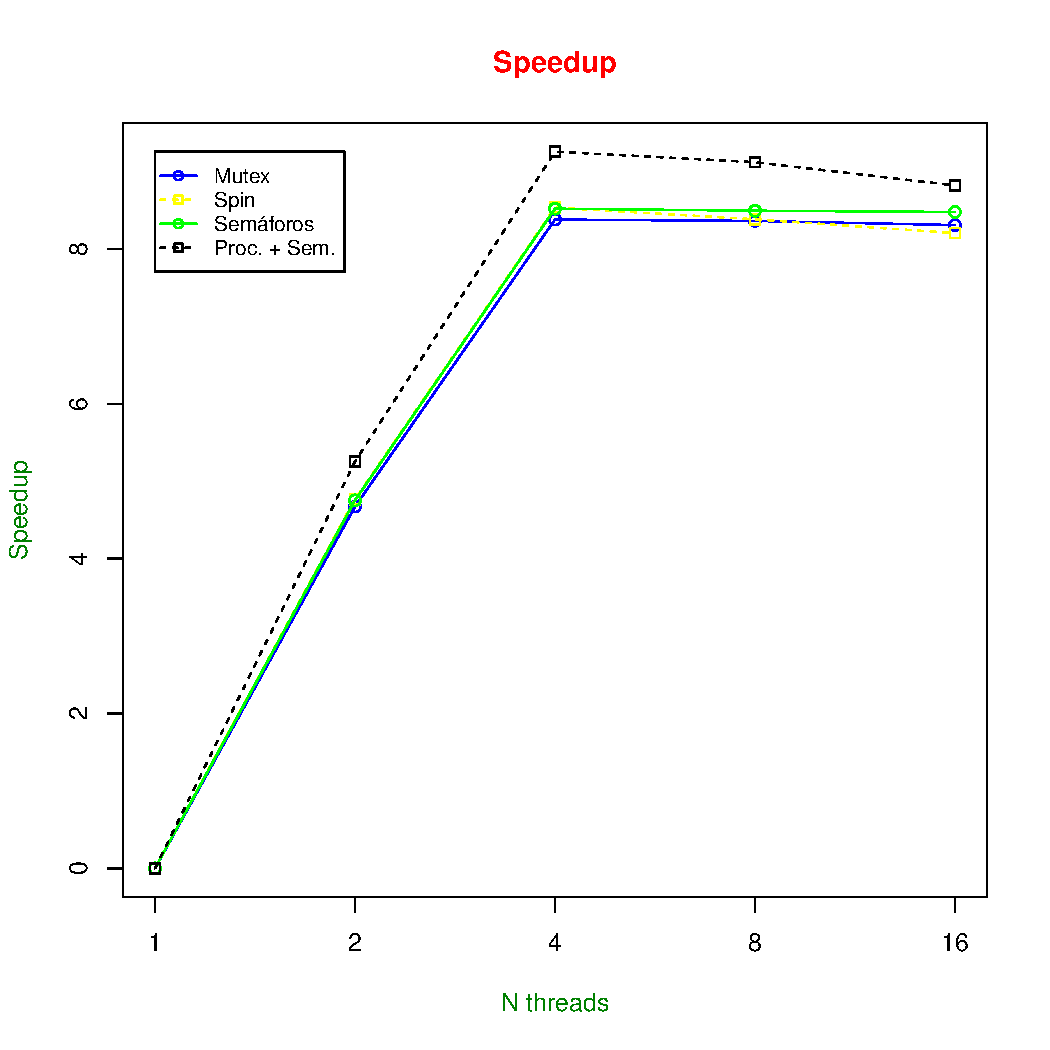
\includegraphics[width=.6\textwidth]{b_sp.pdf}
\caption{Gráfico de speedup}
\label{fig:exampleFig1}
\end{figure}

Principalmente por se tratar de um algoritmo cuja lógica principal é paralela as implementações paralelas de \textit{Barnes} apresentaram resultados bastante expressivos, que se justificam através da independência dos dados em sua execução, possibilitando que cada fluxo de execução trabalhe de maneira semi-contínua, reduzindo drásticamente o tempo de execução total do programa e consequentemente apresentando este speedup.

\begin{figure}[ht]
\centering
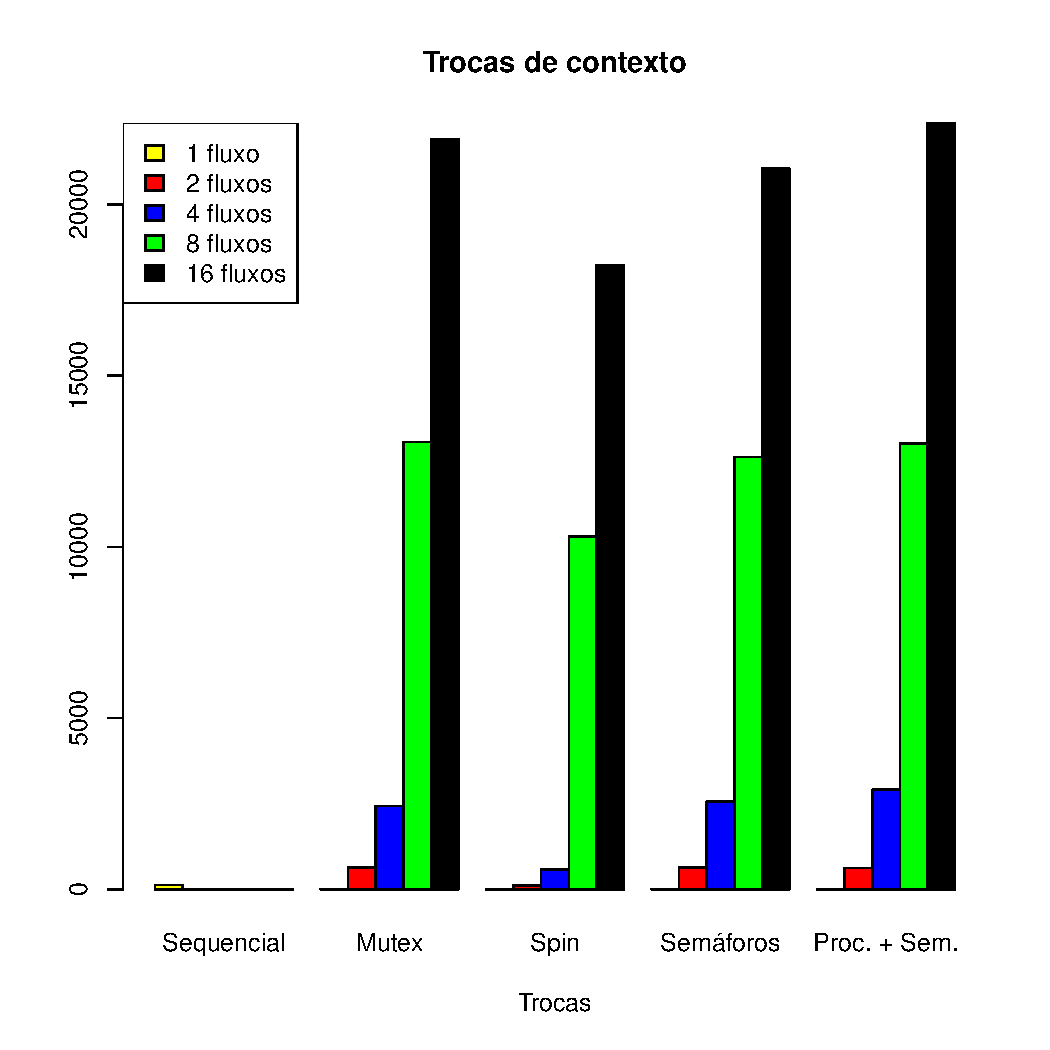
\includegraphics[width=.6\textwidth]{b_ctx.pdf}
\caption{Trocas de contexto}
\label{fig:trocadecontexto}
\end{figure}

Com o gráfico de erros na previsão de desvio (figura 4), podemos ver o principal motivo pelo qual a versão com processos tem maior ganho de desempenho. Por mais que os precessos sejam independentes, a porcentagem de erros é bem menor se comparada à versão com mutex e fica na mesma média das outras versões. Analisando este gráfico com o de erros (misses) na cache de nível mais alto (llc), que está exemplificado na figura 5, podemos ver que a cache é muito mais eficiente no modelo com processos. O índice de acertos na cache é quase igual às outras versões, mas como os acertos na previsão de desvio também são bons, o desempenho no geral é melhor.

\begin{figure}[ht]
\centering
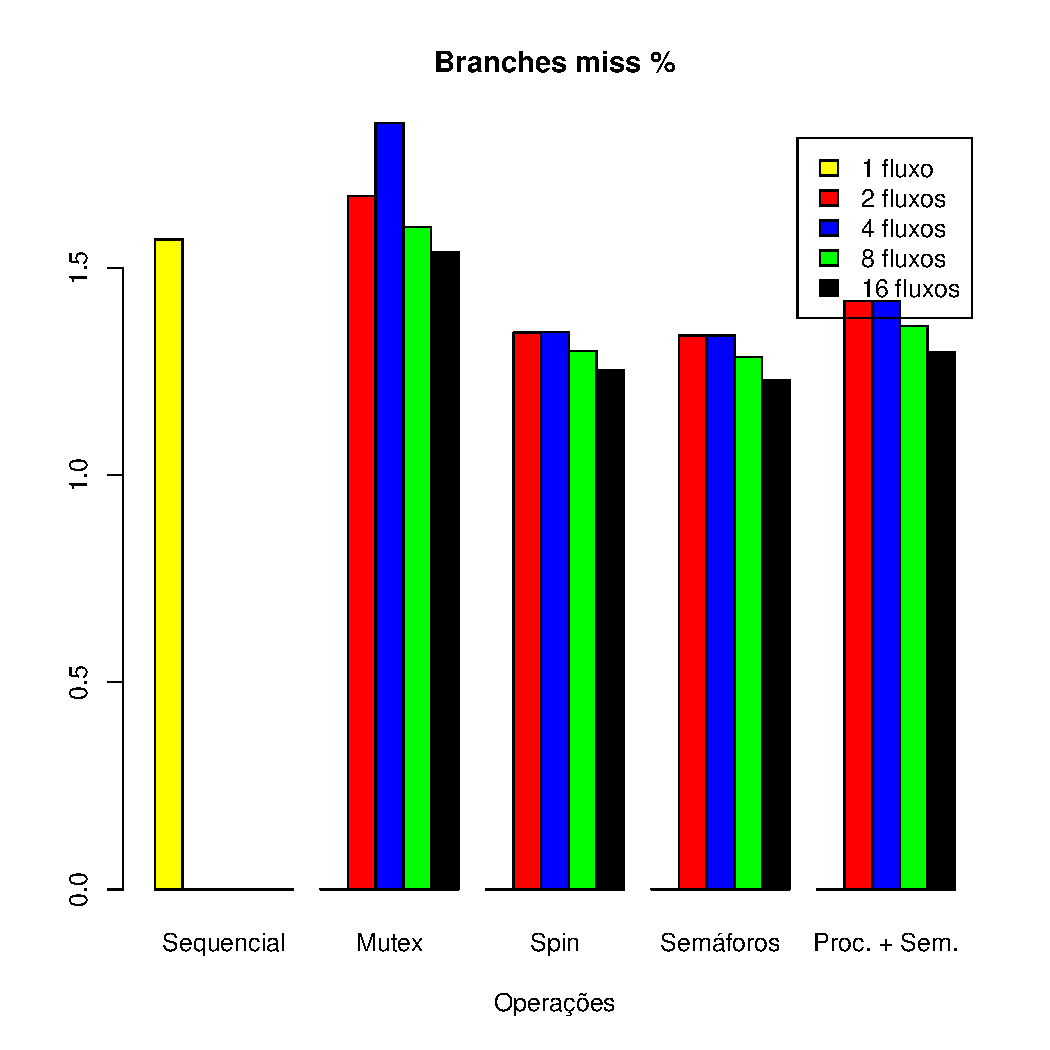
\includegraphics[width=.6\textwidth]{b_bm.pdf}
\caption{Erros na previsão de desvio}
\label{fig:desvios}
\end{figure}

\begin{figure}[ht]
\centering
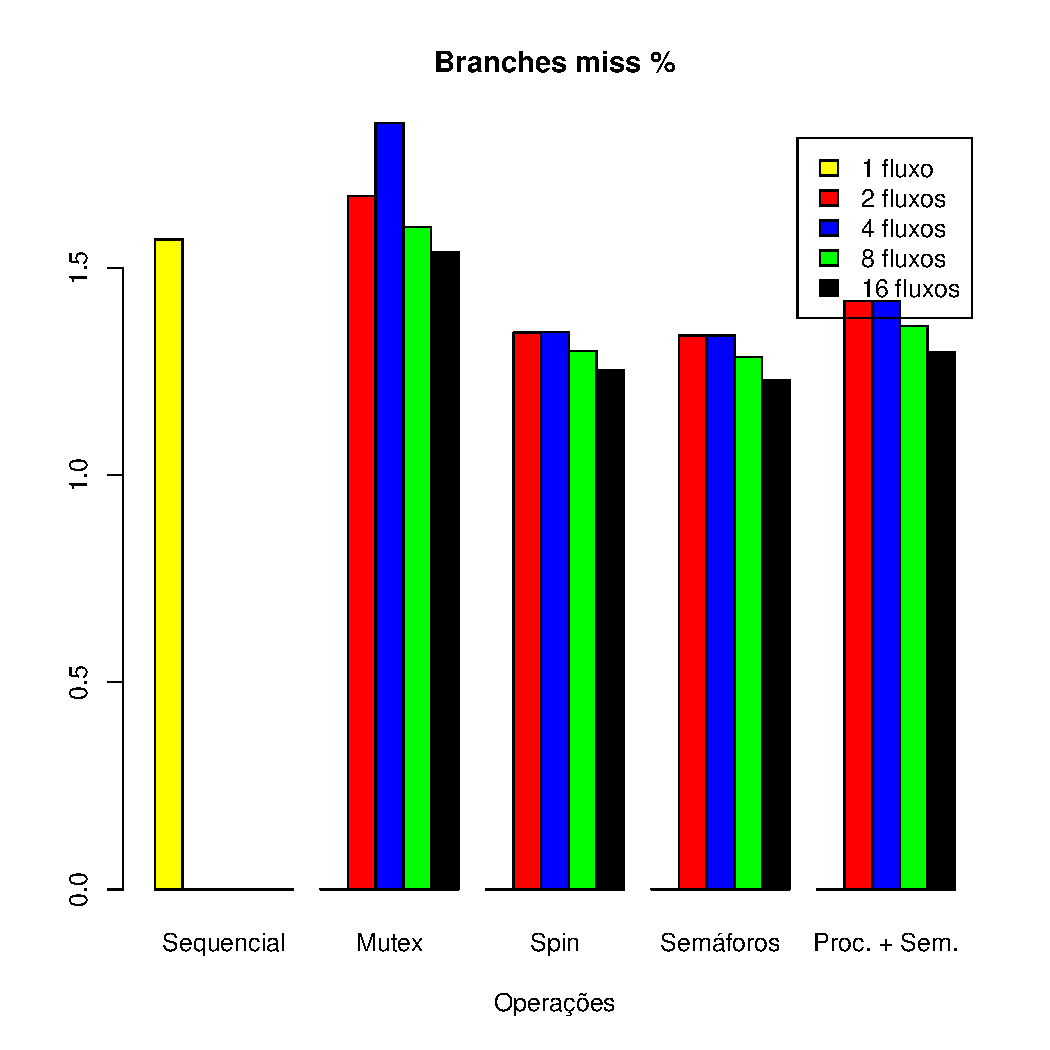
\includegraphics[width=.6\textwidth]{b_bm.pdf}
\caption{Erros na previsão de desvio}
\label{fig:desvios}
\end{figure}

Quanto ao número de trocas de contexto observa-se um contraste muito grande entre a versão sequencial e as implementações paralelas, comportamento já esperado devido a maior permanencia do processo sequencial na CPU e a constante troca de fluxo das versões paralelas. A razão pela qual a quantidade se torna tão maior com 8 e 16 fluxos está na máquina utilizada para os experimentos, como ela possui apenas quatro núcleos as execuções com maior número de fluxos acabam sofrendo uma queda de desempenho devido a troca excessiva de contexto, esta caracteristica também reflete no gráfico de speedup.

\section{Conclusão}
A implementação de algoritmos paralelos pode ser considerada essencial atualmente quando se busca obter programas de alto desempenho, entretanto esta não é uma tarefa fácil e muitas vezes existem barreiras que separam códigos paralelos eficientes e códigos paralelos que não conseguem extrair o potencial do hardware. Algumas vezes estas barreiras se encontram na própria natureza do problema em questão, outras vezes estão na arquitetura da solução em construção, cabe ao programador identificar e lidar com estas limitações. Neste trabalho dois programas distintos foram paralelizados de diversas maneiras, enquanto \textit{Linked List} não apresentou ótimos resultados devido a sua natureza, \textit{Barnes} apresentou bons resultados para todas as implementações, uma delas se destacou: Processos e semáforos obteve os melhores resultados dentre todas implementações. 

\bibliographystyle{sbc}
\bibliography{sbc-template}

\end{document}
